\documentclass{ceurart}

\usepackage{acronym}
\usepackage{subcaption}
\acrodef{3G}[3G]{Third Generation Mobile System}
\acrodef{5S}[5S]{Streams, Structures, Spaces, Scenarios, Societies}
\acrodef{AA}[AA]{Active Agreements}
\acrodef{AAAI}[AAAI]{Association for the Advancement of Artificial Intelligence}
\acrodef{AAL}[AAL]{Annotation Abstraction Layer}
\acrodef{AAM}[AAM]{Automatic Annotation Manager}
\acrodef{AAP}[AAP]{Average Average Precision}
\acrodef{ACLIA}[ACLIA]{Advanced Cross-Lingual Information Access}
\acrodef{ACM}[ACM]{Association for Computing Machinery}
\acrodef{AD}[AD]{Active Disagreements}
\acrodef{ADSL}[ADSL]{Asymmetric Digital Subscriber Line}
\acrodef{ADUI}[ADUI]{ADministrator User Interface}
\acrodef{AIP}[AIP]{Archival Information Package}
\acrodef{AJAX}[AJAX]{Asynchronous JavaScript Technology and \acs{XML}}
\acrodef{ALU}[ALU]{Aritmetic-Logic Unit}
\acrodef{AMUSID}[AMUSID]{Adaptive MUSeological IDentity-service}
\acrodef{ANOVA}[ANOVA]{ANalysis Of VAriance}
\acrodef{ANSI}[ANSI]{American National Standards Institute}
\acrodef{AP}[AP]{Average Precision}
\acrodef{APC}[APC]{AP Correlation}
\acrodef{API}[API]{Application Program Interface}
\acrodef{AR}[AR]{Address Register}
\acrodef{AS}[AS]{Annotation Service}
\acrodef{ASAP}[ASAP]{Adaptable Software Architecture Performance}
\acrodef{ASI}[ASI]{Annotation Service Integrator}
\acrodef{ASL}[ASL]{Achieved Significance Level}
\acrodef{ASM}[ASM]{Annotation Storing Manager}
\acrodef{ASR}[ASR]{Automatic Speech Recognition}
\acrodef{ASUI}[ASUI]{ASsessor User Interface}
\acrodef{ATIM}[ATIM]{Annotation Textual Indexing Manager}
\acrodef{AUC}[AUC]{Area Under the ROC Curve}
\acrodef{AUI}[AUI]{Administrative User Interface}
\acrodef{AWARE}[AWARE]{Assessor-driven Weighted Averages for Retrieval Evaluation}
\acrodef{BANKS-I}[BANKS-I]{Browsing ANd Keyword Searching I}
\acrodef{BANKS-II}[BANKS-II]{Browsing ANd Keyword Searching II}
\acrodef{BH}[BH]{Benjamini-Hochberg}
\acrodef{bpref}[bpref]{Binary Preference}
\acrodef{BNF}[BNF]{Backus and Naur Form}
\acrodef{BPM}[BPM]{Bejeweled Player Model}
\acrodef{BRICKS}[BRICKS]{Building Resources for Integrated Cultural Knowledge Services}
\acrodef{CAN}[CAN]{Content Addressable Netword}
\acrodef{CAS}[CAS]{Content-And-Structure}
\acrodef{CBSD}[CBSD]{Component-Based Software Developlement}
\acrodef{CBSE}[CBSE]{Component-Based Software Engineering}
\acrodef{CB-SPE}[CB-SPE]{Component-Based \acs{SPE}}
\acrodef{CD}[CD]{Collaboration Diagram}
\acrodef{CD}[CD]{Compact Disk}
\acrodef{CDF}[CDF]{Cumulative Density Function}
\acrodef{CENL}[CENL]{Conference of European National Librarians}
\acrodef{CIDOC CRM}[CIDOC CRM]{CIDOC Conceptual Reference Model}
\acrodef{CIR}[CIR]{Current Instruction Register}
\acrodef{CIRCO}[CIRCO]{Coordinated Information Retrieval Components Orchestration}
\acrodef{CG}[CG]{Cumulated Gain}
\acrodef{CL}[CL]{Curriculum Learning}
\acrodef{CL-ESA}[CL-ESA]{Cross-Lingual Explicit Semantic Analysis}
\acrodef{CLAIRE}[CLAIRE]{Combinatorial visuaL Analytics system for Information Retrieval Evaluation}
\acrodef{CLEF1}[CLEF]{Cross-Language Evaluation Forum}
\acrodef{CLEF}[CLEF]{Conference and Labs of the Evaluation Forum}
\acrodef{CLIR}[CLIR]{Cross Language Information Retrieval}
\acrodef{CM}[CM]{Continuation Methods}
\acrodef{CMS}[CMS]{Content Management System}
\acrodef{CMT}[CMT]{Campaign Management Tool}
\acrodef{CNR}[CNR]{Italian National Council of Research}
\acrodef{CO}[CO]{Content-Only}
\acrodef{COD}[COD]{Code On Demand}
\acrodef{CODATA}[CODATA]{Committee on Data for Science and Technology}
\acrodef{COLLATE}[COLLATE]{Collaboratory for Annotation Indexing and Retrieval of Digitized Historical Archive Material}
\acrodef{CP}[CP]{Characteristic Pattern}
\acrodef{CPE}[CPE]{Control Processor Element}
\acrodef{CPU}[CPU]{Central Processing Unit}
\acrodef{CQL}[CQL]{Contextual Query Language}
\acrodef{CRP}[CRP]{Cumulated Relative Position}
\acrodef{CRUD}[CRUD]{Create--Read--Update--Delete}
\acrodef{CS}[CS]{Characteristic Structure}
\acrodef{CSM}[CSM]{Campaign Storing Manager}
\acrodef{CSS}[CSS]{Cascading Style Sheets}
\acrodef{CTR}[CTR]{Click-Through Rate}
\acrodef{CU}[CU]{Control Unit}
\acrodef{CUI}[CUI]{Client User Interface}
\acrodef{CV}[CV]{Cross-Validation}
\acrodef{DAFFODIL}[DAFFODIL]{Distributed Agents for User-Friendly Access of Digital Libraries}
\acrodef{DAO}[DAO]{Data Access Object}
\acrodef{DARE}[DARE]{Drawing Adequate REpresentations}
\acrodef{DARPA}[DARPA]{Defense Advanced Research Projects Agency}
\acrodef{DAS}[DAS]{Distributed Annotation System}
\acrodef{DB}[DB]{DataBase}
\acrodef{DBMS}[DBMS]{DataBase Management System}
\acrodef{DC}[DC]{Dublin Core}
\acrodef{DCG}[DCG]{Discounted Cumulated Gain}
\acrodef{DCMI}[DCMI]{Dublin Core Metadata Initiative}
\acrodef{DCV}[DCV]{Document Cut--off Value}
\acrodef{DD}[DD]{Deployment Diagram}
\acrodef{DDC}[DDC]{Dewey Decimal Classification}
\acrodef{DDS}[DDS]{Direct Data Structure}
\acrodef{DF}[DF]{Degrees of Freedom}
\acrodef{DFI}[DFI]{Divergence From Independence}
\acrodef{DFR}[DFR]{Divergence From Randomness}
\acrodef{DHT}[DHT]{Distributed Hash Table}
\acrodef{DI}[DI]{Digital Image}
\acrodef{DIKW}[DIKW]{Data, Information, Knowledge, Wisdom}
\acrodef{DIL}[DIL]{\acs{DIRECT} Integration Layer}
\acrodef{DiLAS}[DiLAS]{Digital Library Annotation Service}
\acrodef{DIRECT}[DIRECT]{Distributed Information Retrieval Evaluation Campaign Tool}
\acrodef{DKMS}[DKMS]{Data and Knowledge Management System}
\acrodef{DL}[DL]{Digital Library}
\acrodefplural{DL}[DL]{Digital Libraries}
\acrodef{DLMS}[DLMS]{Digital Library Management System}
\acrodef{DLOG}[DL]{Description Logics}
\acrodef{DLS}[DLS]{Digital Library System}
\acrodef{DLSS}[DLSS]{Digital Library Service System}
\acrodef{DM}[DM]{Data Mining}
\acrodef{DO}[DO]{Digital Object}
\acrodef{DOI}[DOI]{Digital Object Identifier}
\acrodef{DOM}[DOM]{Document Object Model}
\acrodef{DoMDL}[DoMDL]{Document Model for Digital Libraries}
\acrodef{DP}[DP]{Discriminative Power}
\acrodef{DPBF}[DPBF]{Dynamic Programming Best-First}
\acrodef{DR}[DR]{Data Register}
\acrodef{DRIVER}[DRIVER]{Digital Repository Infrastructure Vision for European Research}
\acrodef{DTD}[DTD]{Document Type Definition}
\acrodef{DVD}[DVD]{Digital Versatile Disk}
\acrodef{EAC-CPF}[EAC-CPF]{Encoded Archival Context for Corporate Bodies, Persons, and Families}
\acrodef{EAD}[EAD]{Encoded Archival Description}
\acrodef{EAN}[EAN]{International Article Number}
\acrodef{EBU}[EBU]{Expected Browsing Utility}
\acrodef{ECD}[ECD]{Enhanced Contenty Delivery}
\acrodef{ECDL}[ECDL]{European Conference on Research and Advanced Technology for Digital Libraries}
\acrodef{EDM}[EDM]{Europeana Data Model}
\acrodef{EG}[EG]{Execution Graph}
\acrodef{ELDA}[ELDA]{Evaluation and Language resources Distribution Agency}
\acrodef{ELRA}[ELRA]{European Language Resources Association}
\acrodef{EM}[EM]{Expectation Maximization}
\acrodef{EMMA}[EMMA]{Extensible MultiModal Annotation}
\acrodef{EPROM}[EPROM]{Erasable Programmable \acs{ROM}}
\acrodef{EQNM}[EQNM]{Extended Queueing Network Model}
\acrodef{ER}[ER]{Entity--Relationship}
\acrodef{ERR}[ERR]{Expected Reciprocal Rank}
\acrodef{ERS}[ERS]{Empirical Relational System}
\acrodef{ESA}[ESA]{Explicit Semantic Analysis}
\acrodef{ESL}[ESL]{Expected Search Length}
\acrodef{ETL}[ETL]{Extract-Transform-Load}
\acrodef{FAST}[FAST]{Flexible Annotation Service Tool}
\acrodef{FDR}[FDR]{False Discovery Rate}
\acrodef{FIFO}[FIFO]{First-In / First-Out}
\acrodef{FIRE}[FIRE]{Forum for Information Retrieval Evaluation}
\acrodef{FN}[FN]{False Negative}
\acrodef{FNR}[FNR]{False Negative Rate}
\acrodef{FOAF}[FOAF]{Friend of a Friend}
\acrodef{FORESEE}[FORESEE]{FOod REcommentation sErvER}
\acrodef{FP}[FP]{False Positive}
\acrodef{FPR}[FPR]{False Positive Rate}
\acrodef{FWER}[FWER]{Family-wise Error Rate}
\acrodef{GIF}[GIF]{Graphics Interchange Format}
\acrodef{GIR}[GIR]{Geografic Information Retrieval}
\acrodef{GAP}[GAP]{Graded Average Precision}
\acrodef{GLM}[GLM]{General Linear Model}
\acrodef{GLMM}[GLMM]{General Linear Mixed Model}
\acrodef{GMAP}[GMAP]{Geometric Mean Average Precision}
\acrodef{GoP}[GoP]{Grid of Points}
\acrodef{GPRS}[GPRS]{General Packet Radio Service}
\acrodef{gP}[gP]{Generalized Precision}
\acrodef{gR}[gR]{Generalized Recall}
\acrodef{gRBP}[gRBP]{Graded Rank-Biased Precision}
\acrodef{GT}[GT]{Generalizability Theory}
\acrodef{GTIN}[GTIN]{Global Trade Item Number}
\acrodef{GUI}[GUI]{Graphical User Interface}
\acrodef{GW}[GW]{Gateway}
\acrodef{HCI}[HCI]{Human Computer Interaction}
\acrodef{HDS}[HDS]{Hybrid Data Structure}
\acrodef{HIR}[HIR]{Hypertext Information Retrieval}
\acrodef{HIT}[HIT]{Human Intelligent Task}
\acrodef{HITS}[HITS]{Hyperlink-Induced Topic Search}
\acrodef{HMM}[HMM]{Hidden Markov Model}
\acrodef{HTML}[HTML]{HyperText Markup Language}
\acrodef{HTTP}[HTTP]{HyperText Transfer Protocol}
\acrodef{HSD}[HSD]{Honestly Significant Difference}
\acrodef{ICA}[ICA]{International Council on Archives}
\acrodef{ICSU}[ICSU]{International Council for Science}
\acrodef{IDF}[IDF]{Inverse Document Frequency}
\acrodef{IDS}[IDS]{Inverse Data Structure}
\acrodef{IEEE}[IEEE]{Institute of Electrical and Electronics Engineers}
\acrodef{IEI}[IEI]{Istituto della Enciclopedia Italiana fondata da Giovanni Treccani}
\acrodef{IETF}[IETF]{Internet Engineering Task Force}
\acrodef{IIR}[IIR]{Interactive Information Retrieval}
\acrodef{IMS}[IMS]{Information Management System}
\acrodef{IMSPD}[IMS]{Information Management Systems Research Group}
\acrodef{indAP}[indAP]{Induced Average Precision}
\acrodef{infAP}[infAP]{Inferred Average Precision}
\acrodef{INEX}[INEX]{INitiative for the Evaluation of \acs{XML} Retrieval}
\acrodef{INS-M}[INS-M]{Inverse Set Data Model}
\acrodef{INTR}[INTR]{Interrupt Register}
\acrodef{IP}[IP]{Internet Protocol}
\acrodef{IPSA}[IPSA]{Imaginum Patavinae Scientiae Archivum}
\acrodef{IR}[IR]{Information Retrieval}
\acrodef{IRON}[IRON]{Information Retrieval ON}
\acrodef{IRON2}[IRON$^2$]{Information Retrieval On aNNotations}
\acrodef{IRON-SAT}[IRON-SAT]{\acs{IRON} - Statistical Analysis Tool}
\acrodef{IRS}[IRS]{Information Retrieval System}
\acrodef{ISAD(G)}[ISAD(G)]{International Standard for Archival Description (General)}
\acrodef{ISBN}[ISBN]{International Standard Book Number}
\acrodef{ISIS}[ISIS]{Interactive SImilarity Search}
\acrodef{ISJ}[ISJ]{Interactive Searching and Judging}
\acrodef{ISO}[ISO]{International Organization for Standardization}
\acrodef{ITU}[ITU]{International Telecommunication Union }
\acrodef{ITU-T}[ITU-T]{Telecommunication Standardization Sector of \acs{ITU}}
\acrodef{IV}[IV]{Information Visualization}
\acrodef{JAN}[JAN]{Japanese Article Number}
\acrodef{JDBC}[JDBC]{Java DataBase Connectivity}
\acrodef{JMB}[JMB]{Java--Matlab Bridge}
\acrodef{JPEG}[JPEG]{Joint Photographic Experts Group}
\acrodef{JSON}[JSON]{JavaScript Object Notation}
\acrodef{JSP}[JSP]{Java Server Pages}
\acrodef{JTE}[JTE]{Java-Treceval Engine}
\acrodef{KDE}[KDE]{Kernel Density Estimation}
\acrodef{KLD}[KLD]{Kullback-Leibler Divergence}
\acrodef{KLAPER}[KLAPER]{Kernel LAnguage for PErformance and Reliability analysis}
\acrodef{LAM}[LAM]{Libraries, Archives, and Museums}
\acrodef{LAM2}[LAM]{Logistic Average Misclassification}
\acrodef{LAN}[LAN]{Local Area Network}
\acrodef{LD}[LD]{Linked Data}
\acrodef{LEAF}[LEAF]{Linking and Exploring Authority Files}
\acrodef{LIDO}[LIDO]{Lightweight Information Describing Objects}
\acrodef{LIFO}[LIFO]{Last-In / First-Out}
\acrodef{LM}[LM]{Language Model}
\acrodef{LMT}[LMT]{Log Management Tool}
\acrodef{LOD}[LOD]{Linked Open Data}
\acrodef{LODE}[LODE]{Linking Open Descriptions of Events}
\acrodef{LpO}[LpO]{Leave-$p$-Out}
\acrodef{LRM}[LRM]{Local Relational Model}
\acrodef{LRU}[LRU]{Last Recently Used}
\acrodef{LS}[LS]{Lexical Signature}
\acrodef{LSM}[LSM]{Log Storing Manager}
\acrodef{LtR}[LtR]{Learning to Rank}
\acrodef{LUG}[LUG]{Lexical Unit Generator}
\acrodef{MA}[MA]{Mobile Agent}
\acrodef{MA}[MA]{Moving Average}
\acrodef{MACS}[MACS]{Multilingual ACcess to Subjects}
\acrodef{MADCOW}[MADCOW]{Multimedia Annotation of Digital Content Over the Web}
\acrodef{MAD}[MAD]{Mean Assessed Documents}
\acrodef{MADP}[MADP]{Mean Assessed Documents Precision}
\acrodef{MADS}[MADS]{Metadata Authority Description Standard}
\acrodef{MAP}[MAP]{Mean Average Precision}
\acrodef{MARC}[MARC]{Machine Readable Cataloging}
\acrodef{MATTERS}[MATTERS]{MATlab Toolkit for Evaluation of information Retrieval Systems}
\acrodef{MDA}[MDA]{Model Driven Architecture}
\acrodef{MDD}[MDD]{Model-Driven Development}
\acrodef{METS}[METS]{Metadata Encoding and Transmission Standard}
\acrodef{MIDI}[MIDI]{Musical Instrument Digital Interface}
\acrodef{MIME}[MIME]{Multipurpose Internet Mail Extensions}
\acrodef{ML}[ML]{Machine Learning}
\acrodef{MLE}[MLE]{Maximum Likelihood Estimation}
\acrodef{MLIA}[MLIA]{MultiLingual Information Access}
\acrodef{MM}[MM]{Machinery Model}
\acrodef{MMU}[MMU]{Memory Management Unit}
\acrodef{MODS}[MODS]{Metadata Object Description Schema}
\acrodef{MOF}[MOF]{Meta-Object Facility}
\acrodef{MP}[MP]{Markov Precision}
\acrodef{MPEG}[MPEG]{Motion Picture Experts Group}
\acrodef{MRD}[MRD]{Machine Readable Dictionary}
\acrodef{MRF}[MRF]{Markov Random Field}
\acrodef{MRR}[MRR]{Mean Reciprocal Rank}
\acrodef{PRF}[PRF]{Pseudo-Relevance Feedback}
\acrodef{MS}[MS]{Mean Squares}
\acrodef{MSAC}[MSAC]{Multilingual Subject Access to Catalogues}
\acrodef{MSE}[MSE]{Mean Square Error}
\acrodef{MT}[MT]{Machine Translation}
\acrodef{MV}[MV]{Majority Vote}
\acrodef{MVC}[MVC]{Model-View-Controller}
\acrodef{NACSIS}[NACSIS]{NAtional Center for Science Information Systems}
\acrodef{NAP}[NAP]{Network processors Applications Profile}
\acrodef{NCP}[NCP]{Normalized Cumulative Precision}
\acrodef{nCG}[nCG]{Normalized Cumulated Gain}
\acrodef{nCRP}[nCRP]{Normalized Cumulated Relative Position}
\acrodef{nDCG}[nDCG]{Normalized Discounted Cumulated Gain}
\acrodef{nMCG}[nMCG]{Normalized Markov Cumulated Gain}
\acrodef{NESTOR}[NESTOR]{NEsted SeTs for Object hieRarchies}
\acrodef{NEXI}[NEXI]{Narrowed Extended XPath I}
\acrodef{NII}[NII]{National Institute of Informatics}
\acrodef{NISO}[NISO]{National Information Standards Organization}
\acrodef{NIST}[NIST]{National Institute of Standards and Technology}
\acrodef{NLP}[NLP]{Natural Language Processing}
\acrodef{NN}[NN]{Neural Network}
\acrodef{NP}[NP]{Network Processor}
\acrodef{NR}[NR]{Normalized Recall}
\acrodef{NRS}[NRS]{Numerical Relational System}
\acrodef{NS-M}[NS-M]{Nested Set Model}
\acrodef{NTCIR}[NTCIR]{NII Testbeds and Community for Information access Research}
\acrodef{OAI}[OAI]{Open Archives Initiative}
\acrodef{OAI-ORE}[OAI-ORE]{Open Archives Initiative Object Reuse and Exchange}
\acrodef{OAI-PMH}[OAI-PMH]{Open Archives Initiative Protocol for Metadata Harvesting}
\acrodef{OAIS}[OAIS]{Open Archival Information System}
\acrodef{OC}[OC]{Operation Code}
\acrodef{OCLC}[OCLC]{Online Computer Library Center}
\acrodef{OMG}[OMG]{Object Management Group}
\acrodef{OO}[OO]{Object Oriented}
\acrodef{OODB}[OODB]{Object-Oriented \acs{DB}}
\acrodef{OODBMS}[OODBMS]{Object-Oriented \acs{DBMS}}
\acrodef{OPAC}[OPAC]{Online Public Access Catalog}
\acrodef{OQL}[OQL]{Object Query Language}
\acrodef{ORP}[ORP]{Open Relevance Project}
\acrodef{OSIRIS}[OSIRIS]{Open Service Infrastructure for Reliable and Integrated process Support}
\acrodef{P}[P]{Precision}
\acrodef{P2P}[P2P]{Peer-To-Peer}
\acrodef{PA}[PA]{Passive Agreements}
\acrodef{PAMT}[PAMT]{Pool-Assessment Management Tool}
\acrodef{PASM}[PASM]{Pool-Assessment Storing Manager}
\acrodef{PC}[PC]{Program Counter}
\acrodef{PCP}[PCP]{Pre-Commercial Procurement}
\acrodef{PCR}[PCR]{Peripherical Command Register}
\acrodef{PD}[PD]{Passive Disagreements}
\acrodef{PDA}[PDA]{Personal Digital Assistant}
\acrodef{PDF}[PDF]{Probability Density Function}
\acrodef{PDR}[PDR]{Peripherical Data Register}
\acrodef{PIR}[PIR]{Personalized Information Retrieval}
\acrodef{POI}[POI]{\acs{PURL}-based Object Identifier}
\acrodef{PoS}[PoS]{Part of Speech}
\acrodef{PAA}[PAA]{Proportion of Active Agreements}
\acrodef{PPA}[PPA]{Proportion of Passive Agreements}
\acrodef{PPE}[PPE]{Programmable Processing Engine}
\acrodef{PREFORMA}[PREFORMA]{PREservation FORMAts for culture information/e-archives}
\acrodef{PRIMAD}[PRIMAD]{Platform, Research goal, Implementation, Method, Actor, and Data}
\acrodef{PRIMAmob-UML}[PRIMAmob-UML]{mobile \acs{PRIMA-UML}}
\acrodef{PRIMA-UML}[PRIMA-UML]{PeRformance IncreMental vAlidation in \acs{UML}}
\acrodef{PROM}[PROM]{Programmable \acs{ROM}}
\acrodef{PROMISE}[PROMISE]{Participative Research labOratory  for Multimedia and Multilingual Information Systems Evaluation}
\acrodef{pSQL}[pSQL]{propagate \acs{SQL}}
\acrodef{PUI}[PUI]{Participant User Interface}
\acrodef{PURL}[PURL]{Persistent \acs{URL}}
\acrodef{QA}[QA]{Question Answering}
\acrodef{QE}[QE]{Query Expansion}
\acrodef{QoS-UML}[QoS-UML]{\acs{UML} Profile for QoS and Fault Tolerance}
\acrodef{QPA}[QPA]{Query Performance Analyzer}
\acrodef{QPP}[QPP]{Query Performance Prediction}
\acrodef{R}[R]{Recall}
\acrodef{RAM}[RAM]{Random Access Memory}
\acrodef{RAMM}[RAM]{Random Access Machine}
\acrodef{RBO}[RBO]{Rank-Biased Overlap}
\acrodef{RBP}[RBP]{Rank-Biased Precision}
\acrodef{RBTO}[RBTO]{Rank-Based Total Order}
\acrodef{RDBMS}[RDBMS]{Relational \acs{DBMS}}
\acrodef{RDF}[RDF]{Resource Description Framework}
\acrodef{REST}[REST]{REpresentational State Transfer}
\acrodef{REV}[REV]{Remote Evaluation}
\acrodef{RF}[RF]{Relevance Feedback}
\acrodef{RFC}[RFC]{Request for Comments}
\acrodef{RIA}[RIA]{Reliable Information Access}
\acrodef{RMSE}[RMSE]{Root Mean Square Error}
\acrodef{RMT}[RMT]{Run Management Tool}
\acrodef{ROM}[ROM]{Read Only Memory}
\acrodef{ROMIP}[ROMIP]{Russian Information Retrieval Evaluation Seminar}
\acrodef{RoMP}[RoMP]{Rankings of Measure Pairs}
\acrodef{RoS}[RoS]{Rankings of Systems}
\acrodef{RP}[RP]{Relative Position}
\acrodef{RR}[RR]{Reciprocal Rank}
\acrodef{RSM}[RSM]{Run Storing Manager}
\acrodef{RST}[RST]{Rhetorical Structure Theory}
\acrodef{RSV}[RSV]{Retrieval Status Value}
\acrodef{RT-UML}[RT-UML]{\acs{UML} Profile for Schedulability, Performance and Time}
\acrodef{SA}[SA]{Software Architecture}
\acrodef{SAL}[SAL]{Storing Abstraction Layer}
\acrodef{SAMT}[SAMT]{Statistical Analysis Management Tool}
\acrodef{SAN}[SAN]{Sistema Archivistico Nazionale}
\acrodef{SASM}[SASM]{Statistical Analysis Storing Manager}
\acrodef{SBTO}[SBTO]{Set-Based Total Order}
\acrodef{SD}[SD]{Sequence Diagram}
\acrodef{SE}[SE]{Search Engine}
\acrodef{SEBD}[SEBD]{Convegno Nazionale su Sistemi Evoluti per Basi di Dati}
\acrodef{SEM}[SEM]{Standard Error of the Mean}
\acrodef{SERP}[SERP]{Search Engine Result Page}
\acrodef{SFT}[SFT]{Satisfaction--Frustration--Total}
\acrodef{SIL}[SIL]{Service Integration Layer}
\acrodef{SIP}[SIP]{Submission Information Package}
\acrodef{SKOS}[SKOS]{Simple Knowledge Organization System}
\acrodef{SM}[SM]{Software Model}
\acrodef{SME}[SME]{Statistics--Metrics-Experiments}
\acrodef{SMART}[SMART]{System for the Mechanical Analysis and Retrieval of Text}
\acrodef{SoA}[SoA]{Service-oriented Architectures}
\acrodef{SOA}[SOA]{Strength of Association}
\acrodef{SOAP}[SOAP]{Simple Object Access Protocol}
\acrodef{SOM}[SOM]{Self-Organizing Map}
\acrodef{SPARQL}[SPARQL]{Simple Protocol and RDF Query Language}
\acrodef{SPE}[SPE]{Software Performance Engineering}
\acrodef{SPINA}[SPINA]{Superimposed Peer Infrastructure for iNformation Access}
\acrodef{SPLIT}[SPLIT]{Stemming Program for Language Independent Tasks}
\acrodef{SPOOL}[SPOOL]{Simultaneous Peripheral Operations On Line}
\acrodef{SQL}[SQL]{Structured Query Language}
\acrodef{SR}[SR]{Sliding Ratio}
\acrodef{sRBP}[sRBP]{Session Rank Biased Precision}
\acrodef{SRU}[SRU]{Search/Retrieve via \acs{URL}}
\acrodef{SS}[SS]{Sum of Squares}
\acrodef{SSD}[s.s.d.]{statistically significantly different}
\acrodef{SSTF}[SSTF]{Shortest Seek Time First}
\acrodef{STAR}[STAR]{Steiner-Tree Approximation in Relationship graphs}
\acrodef{STON}[STON]{STemming ON}
\acrodef{SVM}[SVM]{Support Vector Machine}
\acrodef{TAC}[TAC]{Text Analysis Conference}
\acrodef{TBG}[TBG]{Time-Biased Gain}
\acrodef{TCP}[TCP]{Transmission Control Protocol}
\acrodef{TEL}[TEL]{The European Library}
\acrodef{TERRIER}[TERRIER]{TERabyte RetrIEveR}
\acrodef{TF}[TF]{Term Frequency}
\acrodef{TFR}[TFR]{True False Rate}
\acrodef{TLD}[TLD]{Top Level Domain}
\acrodef{TME}[TME]{Topics--Metrics-Experiments}
\acrodef{TN}[TN]{True Negative}
\acrodef{TO}[TO]{Transfer Object}
\acrodef{TP}[TP]{True Positve}
\acrodef{TPR}[TPR]{True Positive Rate}
\acrodef{TRAT}[TRAT]{Text Relevance Assessing Task}
\acrodef{TREC}[TREC]{Text REtrieval Conference}
\acrodef{TRECVID}[TRECVID]{TREC Video Retrieval Evaluation}
\acrodef{TTL}[TTL]{Time-To-Live}
\acrodef{UCD}[UCD]{Use Case Diagram}
\acrodef{UDC}[UDC]{Universal Decimal Classification}
\acrodef{uGAP}[uGAP]{User-oriented Graded Average Precision}
\acrodef{UI}[UI]{User Interface}
\acrodef{UML}[UML]{Unified Modeling Language}
\acrodef{UMT}[UMT]{User Management Tool}
\acrodef{UMTS}[UMTS]{Universal Mobile Telecommunication System}
\acrodef{UoM}[UoM]{Utility-oriented Measurement}
\acrodef{UPC}[UPC]{Universal Product Code}
\acrodef{URI}[URI]{Uniform Resource Identifier}
\acrodef{URL}[URL]{Uniform Resource Locator}
\acrodef{URN}[URN]{Uniform Resource Name}
\acrodef{USM}[USM]{User Storing Manager}
\acrodef{VA}[VA]{Visual Analytics}
\acrodef{VAIRE}[VAIR\"{E}]{Visual Analytics for Information Retrieval Evaluation}
\acrodef{VATE}[VATE$^2$]{Visual Analytics Tool for Experimental Evaluation}
\acrodef{VIRTUE}[VIRTUE]{Visual Information Retrieval Tool for Upfront Evaluation}
\acrodef{VD}[VD]{Virtual Document}
\acrodef{VDM}[VDM]{Visual Data Mining}
\acrodef{VIAF}[VIAF]{Virtual International Authority File}
\acrodef{VIM}[VIM]{International Vocabulary of Metrology}
\acrodef{VL}[VL]{Visual Language}
\acrodef{VoIP}[VoIP]{Voice over IP}
\acrodef{VS}[VS]{Visual Sentence}
\acrodef{W3C}[W3C]{World Wide Web Consortium}
\acrodef{WAN}[WAN]{Wide Area Network}
\acrodef{WHO}[WHO]{World Health Organization}
\acrodef{WLAN}[WLAN]{Wireless \acs{LAN}}
\acrodef{WP}[WP]{Work Package}
\acrodef{WS}[WS]{Web Services}
\acrodef{WSD}[WSD]{Word Sense Disambiguation}
\acrodef{WSDL}[WSDL]{Web Services Description Language}
\acrodef{WWW}[WWW]{World Wide Web}
\acrodef{XMI}[XMI]{\acs{XML} Metadata Interchange}
\acrodef{XML}[XML]{eXtensible Markup Language}
\acrodef{XPath}[XPath]{XML Path Language}
\acrodef{XSL}[XSL]{eXtensible Stylesheet Language}
\acrodef{XSL-FO}[XSL-FO]{\acs{XSL} Formatting Objects}
\acrodef{XSLT}[XSLT]{\acs{XSL} Transformations}
\acrodef{YAGO}[YAGO]{Yet Another Great Ontology}
\acrodef{YASS}[YASS]{Yet Another Suffix Stripper}

\renewcommand{\acffont}[1]{\textsl{#1}}


%%
%% end of the preamble, start of the body of the document source.
\begin{document}
\bibliographystyle{plainnat}
\bibliography{bibliography}
%%
%% Rights management information.
%% CC-BY is default license.
\copyrightyear{2026}
\copyrightclause{Copyright for this paper by its authors.\\
  Use permitted under Creative Commons License Attribution 4.0
  International (CC BY 4.0).}

%%
%% This command is for the conference information
\conference{``Search Engines'', course at the master degree in ``Computer Engineering'', Department of Information Engineering, and at the master degree in ``Data Science'', Department of Mathematics ``Tullio Levi-Civita'', University of Padua, Italy. Academic Year 2025/2026}

%%
%% The "title" command
\title{SEUPD@CLEF: Team DSPY}

%%
%% The "author" command and its associated commands are used to define
%% the authors and their affiliations.
\author[1]{Carlo Galiano}[%
email=carlo.galiano.1@studenti.unipd.it
]

\author[1]{Alberto Iurlo}[%
email=alberto.iurlo@studenti.unipd.it
]

\author[1]{Stefano Riato}[%
email=stefano.riato@studenti.unipd.it
]

\address[1]{University of Padua, Italy}


%%
%% The abstract is a short summary of the work to be presented in the
%% article.
\begin{abstract}
  This paper presents Team DSPY's Information Retrieval (IR) system for the CLEF 2026 CheckThat! Lab Task 1, 
  where the main goal is to retrieve scientific publications for multilingual social media claims. 
  The primary challenge is the high degree of vocabulary mismatch between short multilingual tweets and long technical abstracts 
  centered on English. As such, the development of our system goes beyond the initial baseline algorithm (i.e. BM25) 
  to a sophisticated neural architecture. As the results of empirical analysis suggested that statistical query expansion 
  (Pseudo-Relevance Feedback) suffers from topic drift, we designed an \textbf{Asymmetric Hybrid Search Pipeline}. 
  This novel approach routes English queries through a highly-tuned lexical engine, while reserving computationally expensive 
  long-context dense retrieval (BGE-M3) and Cross-Encoder semantic re-ranking strictly for the processing of French and German queries. 
  The proposed solution has proved to be efficient in terms of the averaged MRR@5 score.
\end{abstract}

%%
%% Keywords. The author(s) should pick words that accurately describe
%% the work being presented. Separate the keywords with commas.
\begin{keywords}
  keyword 1 \sep
  keyword 2 \sep
  keyword 3 
\end{keywords}

%%
%% This command processes the author and affiliation and title
%% information and builds the first part of the formatted document.
\maketitle


\section{Introduction}
\label{sec:introduction}
This report aims to provide a brief explanation of the Information Retrieval system built for Task 1. This paper aims to share the experiments, the analysis, and the results obtained  during the course of the one month in order to compete in the CheckThat!~Lab Task~1 competition. 

The CLEF~2026 CheckThat!~Lab Task~1 frames scientific claim retrieval as
a low-resource, cross-lingual ad-hoc retrieval problem~\citet{hafid2025}.
As shown in Figure~\ref{fig:task-definition}, given a social media post (e.g. tweet) that implicitly cites a scientific
paper, mainly in English, German, or French, containing opinions, comments, hashtags, or tags, the system must rank a fixed corpus of 10{,}000~scientific papers so that the cited paper appears as high as possible in the returned list.
The task is challenging for two reasons: (i)~tweets are short, noisy, and
multilingual, while scientific abstracts are long, technical, and predominantly
written in English; and (ii)~a German or French query may
correspond to an English target paper, so monolingual retrieval breaks
the assumption that query and document share a vocabulary.


We approach this problem as an opportunity to systematically apply and 
evaluate core IR techniques — from sparse lexical models to dense 
neural retrieval — against a real-world competitive benchmark.
Our experiments investigate the trade-offs between retrieval 
effectiveness and computational efficiency under the constraints imposed 
by the competition setting.

\begin{figure}
  \centering
  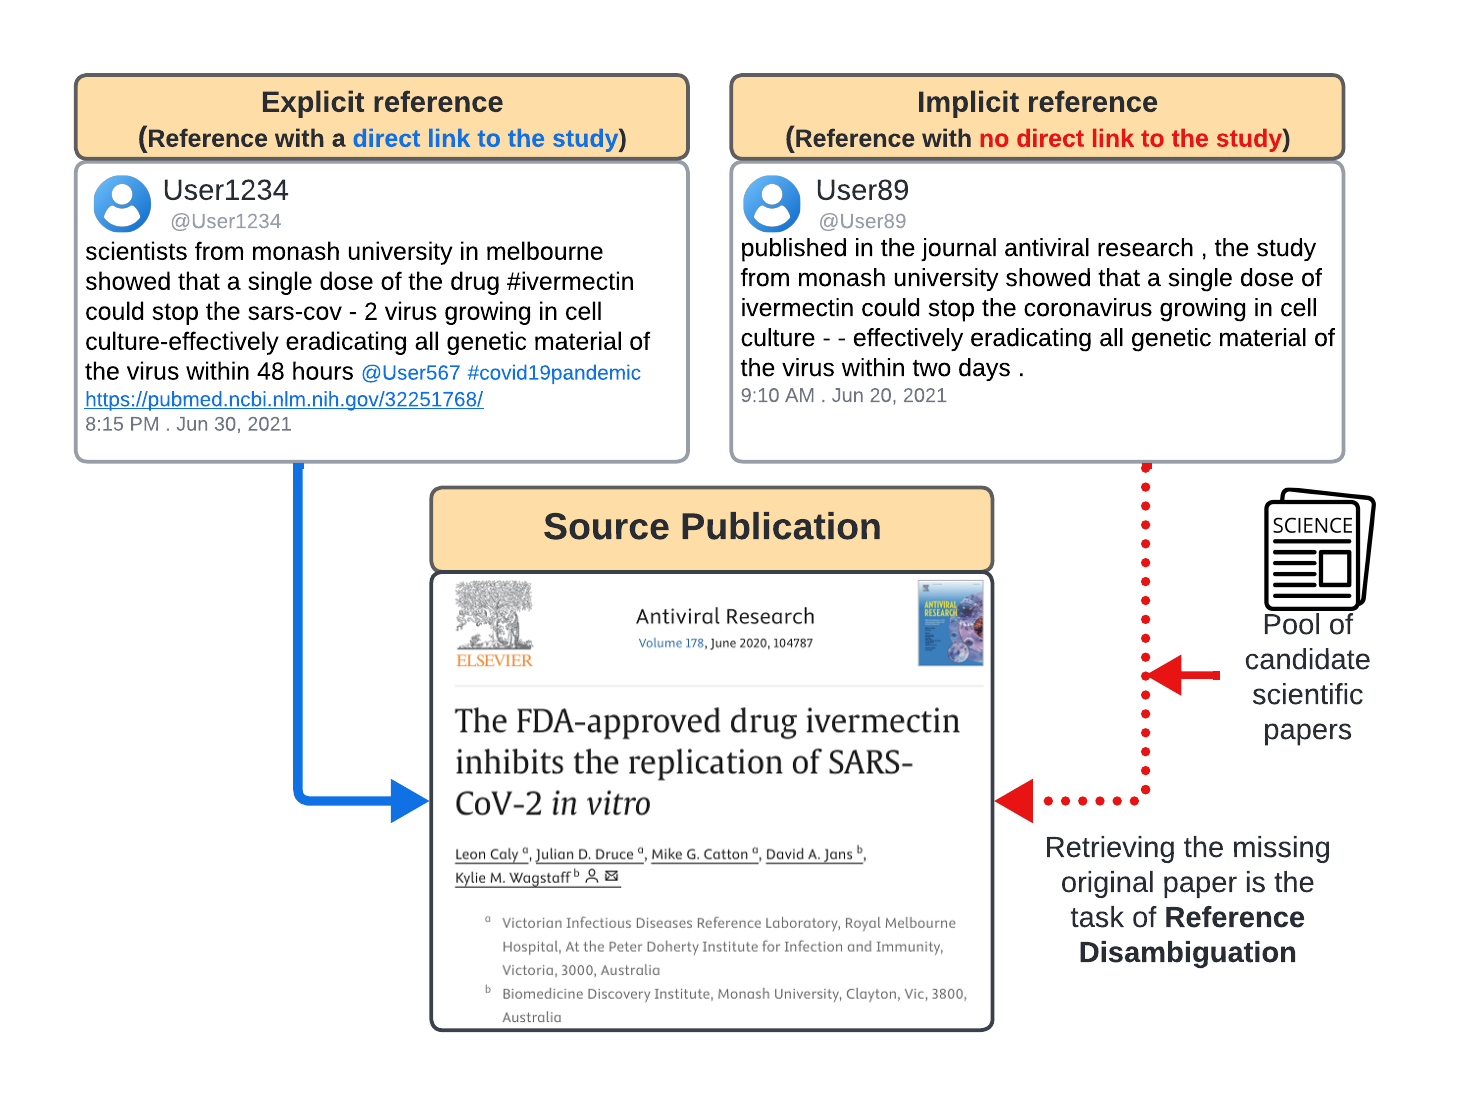
\includegraphics[width=0.6\linewidth]{figure/01-figure_example-task.png}
  \caption{Source Retrieval for Scientific Web Claims problem [Public Domain], 
  it shows a claim with an implicit reference for which the source publication (box to the right) 
  needs to be retrieved in task 4b (adapted from \citet{hafid2025})}
  \label{fig:task-definition}
\end{figure}

The paper is organized as follows: Section~\ref{sec:methodology} describes our approach; 
Section~\ref{sec:setup} explains our experimental setup; Section~\ref{sec:results} discusses our main findings and problems; 
finally, Section~\ref{sec:conclusion} draws some conclusions and outlooks for future work.

\input{section/related-worked}

\section{Methodology}
\label{sec:methodology}

Describe the methodology you have adopted, the architecture of your system, your workflow, etc.



\subsection{Document and Query Parsing}

Documents and queries are parsed through dedicated classes that implement
the Python iterator protocol, allowing the system to process the files sequentially without loading the whole collection into memory in one step.



\subsubsection{Document Parsing}
The \texttt{JsonArrayDocumentParser} reads the data collection in sets of
500 documents. For each document, the title and abstract are concatenated together and passed to the \texttt{langdetect} library to assign a language label (\texttt{en}, \texttt{de}, \texttt{fr}, or \texttt{other}).
Each document in the collection is coded as a \texttt{ParsedDocument} object
carrying its ID, title, abstract, and detected language (which will be later used to determine the analyzer in the indexing phase).

\subsubsection{Query Parsing}
Queries are parsed by the \texttt{JsonArrayQueryParser}, which follows the
same pattern built for document parsing. Since being social media tweets and not scientific paper as in the case of the documents, queries are "cleaned":
mentions, URLs, and hashtag symbols are removed while alphanumeric content and essential punctuation are kept. Moreover, the \texttt{extract\_entities()} method scans each quary looking for the presence of scientific journal names from \texttt{journals.txt}; if the match has a positive correspondence, in searching phase documents published on that journal will get a boost.
An important difference to bring to light regarding the language detection: queries are partitioned for language, hence no language tag is assigned to them.


\subsection{Data Preprocessing}
The linguistic textual preprocessing, both for documents and queries, is executed through the Lucene's built-in analyzers:
\begin{itemize}
    \item \item \texttt{EnglishAnalyzer} — tokenization, lowercase conversion, English stopword removal, and Porter stemming
    \item \texttt{GermanAnalyzer} — tokenization, lowercase conversion, 
German stopword removal, and Snowball stemming
    \item \texttt{FrenchAnalyzer} — tokenization, lowercase conversion, 
French stopword removal, and French light stemming
    \item \texttt{StandardAnalyzer} — tokenization and lowercase 
    conversion only, used as a fallback for other languages with no query correspondence (Italian and Spanish)
\end{itemize}

\subsubsection{Regular Expressions}
The very first textual preprocessing applied was "manually" built since relied on:
\begin{itemize}
    \item lowercase conversion to ensure case-insensitive matching.
    \item regular expression for tokenization and HTML tag removal. In detail \texttt{re.sub(r'<[{\textasciicircum}]+>', '', text)} 
    to strip HTML tags and \texttt{RegexpTokenizer(r'[A-Za-z0-9\%\textbackslash.\textbackslash-]+')} 
    to extract only alphanumeric tokens, percentages, and hyphenated 
    compounds such as \textit{SARS-CoV-2}.
    \item the NLTK library for Snowball stemming and stopword removal
\end{itemize}

This approach was discarded because of two reasons, the first one related to the risk of mismatching between document and query indexing, and - more importantly - the run score obtained with the manual approach was less effective than those achieved using Lucene's analyzers.

An early preprocessing approach explored during development relied on 
a custom \texttt{TextProcessor} class built on top of NLTK. For each 
document or query, the pipeline applied HTML tag removal via regular 
expressions, tokenisation through a \texttt{RegexpTokenizer} 
(\texttt{[A-Za-z0-9\%\textbackslash.\textbackslash-]+}), stopword 
removal, and Snowball stemming — all handled explicitly in Python for 
English, French, and German.




\subsection{Embeddings}
As mentioned previously, our information retrieval pipeline built exploits embeddings. To clarify how the are used it is necessary to make a  distinction between \textbf{sparse} and \textbf{dense} embeddings. 
\textit{Sparse} embeddings are high-dimensional vectors in which the majority of elements are 0, making them computationally lightweight. These vectors do not catch any sentence meaning, and therefore they are suitable for exact-matching task. On the other hand, \textit{Dense} embeddings are low-dimensional vectors, where each dimension carries a fragment of semantic meaning. In detail, the contextual embeddings created with the model
paraphrase-multilingual-MiniLM-L12-v2 are \textit{contextual}, allowing the retrieval of information that goes beyond the "vocabulary mismatch".



\subsection{Pseudo-Relevance Feedback}
One of the runs was obtained by augmenting the baseline through \textbf{Pseudo-Relevance Feedback} (PRF), with the intent of reducing the vocabulary mismatch between documents and queries (written as informal social media posts).

\textit{Pseudo-Relevance Feedback} is a query expansion technique that enriches the query using the vocabulary of the top ranked documents retrieved. The strong assumption, on which the technique relies, lies in the relevance of the documents retrieved using the BM25 model.

In our system, PRF works as a two stage process. In the part the query is executed and the top 3 documents are retrieved; their title and abstract are concatenated and processed in order to extract the 5 most frequent tokens (non stopword with a minimal length of 4 characters). In the second stage, these terms are added alongside the original query as \textbf{SHOULD} clause, so that PRF can only boost a document without excluding those only  matching the original query.

However, this approach did not lead to the expected improvements: the score produced was lower than the baseline obtained using the BM25 model. The likely reason is that PRF's effectiveness strongly depends on the quality of the initial retrieval - if the top ranked documents retrieved are not relevant, the query expansion introduces a lot of noise causing a phenomenon called \textit{query drift}. 


\section{Experimental Setup}
\label{sec:setup}

\subsection{Document Collection and Queries}
\label{subsec:collection}

\paragraph{Document corpus.}
The document collection consists of 10{,}000 scientific publications 
provided by the CLEF~2026 CheckThat!~Lab Task~1 organisers.
Each publication is described by the following metadata fields: 
\texttt{title}, \texttt{abstract}, \texttt{authors}, \texttt{venue}, 
and a unique identifier \texttt{pubkey}.
In our system, we index only the \texttt{title} and \texttt{abstract} 
fields, as these carry the core semantic content of a paper and are 
available for all documents in the corpus.

\paragraph{Query sets.}
The queries consist of short social media posts (tweets), partitioned 
into three official splits: training, development, and test.
Each query is provided as a \texttt{text} field containing the raw 
social media content, along with a \texttt{pubkey} field that identifies 
the single relevant document in the corpus.
This yields a \textit{one-to-one relevance mapping}: each query is 
associated with exactly one ground-truth document, making this a 
highly precise but recall-agnostic retrieval setting.

Table~\ref{tab:collection} summarises the statistics of the collection 
and query splits.
\begin{table}[h]
  \caption{Collection and query statistics.}
  \label{tab:collection}
  \centering
  \begin{tabular}{lrrr}
    \toprule
    Split & English & German & French \\
    \midrule
    Train queries & 14977 & 1460 & 2807 \\
    Dev queries   & 3905 & 386 & 702 \\
    Test queries  & 6080 & 876 & 1220 \\
    \midrule
    Corpus documents & \multicolumn{3}{c}{10{,}000} \\
    \bottomrule
  \end{tabular}
\end{table}

\subsection{Evaluation Measures}
\label{subsec:measures}

We evaluate retrieval quality using the official metric \ac{MRR}@5, which rewards
systems that place the single relevant document in the top-5 ranked positions.
In addition, we report \ac{MAP}, \ac{NDCG}@10, Precision@1, and Recall@1000 to
characterise different aspects of ranking quality.
Evaluation is performed with the \texttt{ranx} library using relevance
judgements (\texttt{qrels}) derived from the ground-truth \texttt{pubkey} labels
provided with each query.

\subsection{Repository}
\label{subsec:repo}

The source code is publicly available at:
\url{https://bitbucket.org/upd-dei-stud-prj/seupd2526-dspy/src/master/}.
%
The repository is organised as follows:
\begin{itemize}
  \item \texttt{pylucene/src/} — entry point orchestrator (\texttt{runner.py}) and data acquisition scripts.
  \item \texttt{pylucene/src/Index/} — core PyLucene and FAISS indexing pipelines (\texttt{index.py}, \\ \texttt{index\_faiss.py}).
  \item \texttt{pylucene/src/Search/} — core execution scripts for the four retrieval methodologies \\(\texttt{search\_v1.py} to \texttt{search\_v4.py}).
  \item \texttt{pylucene/src/Parse/} — data pre-processing and formatting classes for documents and queries.
  \item \texttt{pylucene/src/Evaluation/} \& \texttt{utils/} — scoring (\texttt{evaluate.py}), report generation, ground truth creation, and submission formatting.
  \item \texttt{experiment/} — generated artefacts (index, runs, qrels); not committed to version control.
\end{itemize}

\subsection{Hardware and Software}
\label{subsec:hardware}

Experiments were conducted on three machines. All ran the retrieval pipeline
inside a Docker container built from the official \texttt{coady/pylucene} image,
which bundles PyLucene~9 (Lucene~9.x) on Python~3.11 (to check).

\begin{table}[h]
  \caption{Hardware specifications of the development machines.}
  \label{tab:hardware}
  \centering
  \begin{tabular}{llll}
    \toprule
    Component & Machine~1 & Machine~2 & Machine~3 \\
    \midrule
    CPU & Intel Core i5-13420H  & AMD Ryzen AI 7 350    & Intel Core i7-6500U   \\
        & (13th Gen)            &                       & @ 2.50\,GHz           \\
    RAM & 32\,GB DDR5 5600\,MHz & 16\,GB DDR5 5600\,MHz & 12\,GB DDR4 2133\,MHz \\
    GPU & Intel UHD Graphics    & AMD Radeon 860M +     & NVIDIA GeForce 920MX  \\
        &                       & NVIDIA RTX~5060 Laptop&                       \\
    OS  & Windows~11 Home       & Windows~11 Home       & Windows~10 Home       \\
    \bottomrule
  \end{tabular}
\end{table}

The Docker environment also exposes a Jupyter notebook server on port~8888 for Exploratory Data Analysis. The GPU of Machine~2 was used to accelerate the neural cross-encoder re-ranker (\texttt{rerank.py}) and FAISS dense retrieval experiments (\texttt{index\_faiss.py} and \texttt{search\_faiss.py}). All BM25 indexing , and \ac{PRF}  are fully reproducible on \ac{CPU} and were run on all three machines.


\section{Experimental Results}
\label{sec:results}

This section presents the quantitative evaluation of the four runs in the development and training phases. The results highlight how each architectural decision was motivated by the limitations witnessed in the previous system.


\subsection{V1 — BM25 Baseline}

V1 is the starting reference point for all subsequent runs. As shown in 
Table~\ref{tab:dev_macro}, it achieves an average MRR@5 of 0.2190, a MAP of 0.2322, and an NDCG@10 of 0.2488 on the development set. The per-language division in Table~\ref{tab:dev_lang} displays a strong imbalance among the languages: English reaches MRR@5 = 0.4910, while German and French respectively have the scores 0.0968 and 0.0691. This huge gap suggests that the baseline is competitive for English, but much less effective in the multilingual setting addressed by the task. In the training set, the same pattern remains visible. Table~\ref{tab:train_macro} shows that V1 reaches an average MRR@5 of 0.2301, MAP of 0.2437, and NDCG@10 of 0.2606, while Table~\ref{tab:train_lang} reports MRR@5 values of 0.5028 for English, 0.0970 for German, and 0.0904 for French. The consistency between development and training results highlights that the main limitation of V1 is structural rather than split-specific, and therefore motivates the search for a system that can improve non English queries retrieval.


\subsection{V2 — Pseudo-Relevance Feedback}

V2 was the first system developed as an attempt to improve the baseline retrieval , but as previously anticipated, the results show a consistent deterioration. In the development set, Table~\ref{tab:dev_macro} shows that average MRR@5 decreases from 0.2190 in V1 to 0.1892 in V2, while MAP drops from 0.2322 to 0.2011 and NDCG@10 from 0.2488 to 0.2185. The same trend repeated itself in the training set, where average MRR@5 falls from 0.2301 to 0.1971, MAP from 0.2437 to 0.2102, and NDCG@10 from 0.2606 to 0.2284 (Table~\ref{tab:train_macro}).

\noindent The per language results confirm that the decreasing is not attributable to a single language. In the development set (Table~\ref{tab:dev_lang}), English MRR@5 goes down from 0.4910 to 0.4285, German from 0.0968 to 0.0806, and French from 0.0691 to 0.0585. A similar pattern is observed in the training set (Table~\ref{tab:train_lang}), where all three language specific values remain below those of V1. Since V2 metrics are inferior with respect to the baseline, it was necessary to continue the search of a better performing model


\subsection{V3 — Hybrid Asymmetric Search}

V3 represents the first substantial improvement over the baseline system. In the development set, Table~\ref{tab:dev_macro} shows that average MRR@5 increases to 0.3913, with MAP reaching 0.4054 and NDCG@10 rising to 0.4277. Compared to V1 and V2, this is a clear breakthrough in all three metrics. The same result is confirmed by the training set, where V3 achieves the best scores among the evaluated runs: 
MRR@5 = 0.3957, MAP = 0.4103, and NDCG@10 = 0.4318 (Table~\ref{tab:train_macro}). 
\noindent The language results clarify where this achievement comes from, bringing to light that the gain is completely driven by the hybrid dense-sparse retrieval introduced. In the development set (Table~\ref{tab:dev_lang}), English matches V1 at 0.4910, while German and French improve significantly from 0.0968 to 0.2919 and from 0.0691 to 0.3910, respectively. The same behavior is observable in the training set (Table~\ref{tab:train_lang}), where English remains at 0.5028, while German increases to 0.2906 and French to 0.3937. The results obtained show that the new formulation highly improves the retrieval over German and French, achieving an overall better performance. Nevertheless, the gap between English and the other two languages suggested that the Max-P chunking strategy used was causing the fragmentation of the long semantic dependence, 
justifying the search for another model.

\subsection{V4 — SOTA Hybrid Architecture}

V4 achieves the best results on the development set and represents the final retrieval system formulation. As shown in Table~\ref{tab:dev_macro}, it reaches an average MRR@5 of 0.4919, a MAP of 0.5038, and an NDCG@10 of 0.5298, outperforming all previous runs on every metric. In detail, the jump from V3 to V4 is remarkable, gaining 10 percentage points over the three metrics.
\noindent The per language results in Table~\ref{tab:dev_lang} show that V4 is also the most balanced system among the languages. English decreases a bit to 0.4898, which is really close to the best previous English results, while German increases to 0.4382 and French to 0.5476. Compared to V3, this means a substantial gain from 0.2919 to 0.4382 in German and from 0.3910 to 0.5476 in French. These results confirm that switching to \texttt{BAAI/bge-m3} and eliminating the Max-P chunking strategy (Section~\ref{subsec:methodology_v4}) was the key architectural decision to overcome the weakness related to the metrics' gap among the languages.


\subsection{Results Tables}

\newcolumntype{C}{>{\centering\arraybackslash}X}
\newcolumntype{R}{>{\raggedright\arraybackslash}p{5.8cm}}

\begin{table}[H]
\centering
\caption{Averaged results on the development set.}
\begin{tabularx}{\textwidth}{RCCC}
\toprule
\textbf{Run} & \textbf{MRR@5} & \textbf{MAP} & \textbf{NDCG@10} \\
\midrule
V4 — SOTA Hybrid (bge-m3 + CE)   & \textbf{0.4919} & \textbf{0.5038} & \textbf{0.5298} \\
V3 — Hybrid Asymmetric (e5 + CE) & 0.3913          & 0.4054          & 0.4277          \\
V1 — BM25 Baseline               & 0.2190          & 0.2322          & 0.2488          \\
V2 — BM25 + PRF                  & 0.1892          & 0.2011          & 0.2185          \\
\bottomrule
\end{tabularx}
\label{tab:dev_macro}  %questi sono i nomi delle tabelle da citare per l'interazione
\end{table}

\begin{table}[H]
\centering
\caption{Per-language metrics result in the development set.}
\begin{tabularx}{\textwidth}{RCCCC}
\toprule
\textbf{Run} & \textbf{EN} & \textbf{DE} & \textbf{FR} & \textbf{Avg} \\
\midrule
V4 — SOTA Hybrid (bge-m3 + CE)   & 0.4898          & \textbf{0.4382}          & \textbf{0.5476} & \textbf{0.4919} \\
V3 — Hybrid Asymmetric (e5 + CE) & \textbf{0.4910} & 0.2919          & 0.3910          & 0.3913          \\
V1 — BM25 Baseline               & \textbf{0.4910} & 0.0968          & 0.0691          & 0.2190          \\
V2 — BM25 + PRF                  & 0.4285          & 0.0806          & 0.0585          & 0.1892          \\
\bottomrule
\end{tabularx}
\label{tab:dev_lang} %questi sono i nomi delle tabelle da citare per l'interazione
\end{table}

\begin{table}[H]
\centering
\caption{Averaged results on the training set.}
\begin{tabularx}{\textwidth}{RCCC}
\toprule
\textbf{Run} & \textbf{MRR@5} & \textbf{MAP} & \textbf{NDCG@10} \\
\midrule
V3 — Hybrid Asymmetric (e5 + CE) & \textbf{0.3957} & \textbf{0.4103} & \textbf{0.4318} \\
V1 — BM25 Baseline               & 0.2301          & 0.2437          & 0.2606          \\
V2 — BM25 + PRF                  & 0.1971          & 0.2102          & 0.2284          \\
\bottomrule
\end{tabularx}
\label{tab:train_macro} %questi sono i nomi delle tabelle da citare per l'interazione
\end{table}

\begin{table}[H]
\centering
\caption{Per-language metrics result in the training set}
\begin{tabularx}{\textwidth}{RCCCC}
\toprule
\textbf{Run} & \textbf{EN} & \textbf{DE} & \textbf{FR} & \textbf{Avg} \\
\midrule
V3 — Hybrid Asymmetric (e5 + CE) & \textbf{0.5028} & \textbf{0.2906} & \textbf{0.3937} & \textbf{0.3957} \\
V1 — BM25 Baseline               & \textbf{0.5028} & 0.0970          & 0.0904          & 0.2301          \\
V2 — BM25 + PRF                  & 0.4377          & 0.0795          & 0.0742          & 0.1971          \\
\bottomrule
\end{tabularx}
\label{tab:train_lang} %questi sono i nomi delle tabelle da citare per l'interazione
\end{table}





\section{Conclusions and Future Work}
\label{sec:conclusion}

This paper presented four retrieval systems developed for the Scientific Retrieval task proposed by CLEF, addressing the challenge of matching 
informal social media queries to multilingual scientific documents in English, French, and German.
\noindent Our experiments expose a consistent progression in retrieval achievement (measured as scores of the metrics used) across the runs. The baseline, if on one hand established the upper bound for English queries, on the other hand highlighted the structural limits of an exact matching system based; indeed, the vocabulary mismatch between informal social media posts and scientific documents caused the collapse of the metrics scores for German and French.  The attempt to address this gap through the query expansion technique Pseudo Relevance Feedback has further decreased the scores, confirming the poor quality of the initial retrieval set. The introduction of hybrid dense-sparse retrieval through FAISS, combined 
with a Cross-Encoder re-ranker, produced a first substantial increment in the retrieval of non English queries; indeed, the deep neural networks used for German and French allowed the retrieval of documents thanks to the semantic embeddings similarity. 
\noindent The final architecture refined the hybrid pipeline by using a more powerful long-context retrieval model, which eliminated the previous chunking need. The results achieved were the highest and most balanced across all three languages, confirming that the hybrid dense-sparse retrieval with a neural re-ranking represents the most effective architecture for multilingual scientific document retrieval in this setting.

\section{Group Members Contribution}

% For each group member, describe in detail the contribution to the project.

\begin{description}
	\item[Carlo Galiano] helped with the initial infrastructure setup, developing the dataset acquisition scripts and the data parsers with language detection capabilities (langdetect library). He engineered the core retrieval pipelines, starting from the multi-field BM25 lexical baseline with tuned hyperparameters and native multilingual analyzers, up to Cross-Encoder semantic re-ranking. Furthermore, he implemented the evaluation framework using the \texttt{ranx} library, developed the automated user-friendly script (\texttt{runner.py}), and contributed to the drafting of the Methodology sections of this paper.
	\item[Alberto Iurlo] On the implementation side, the contribution consisted in: document parsing, text processing, boosting different query fields, bug fixing in the retrieval pipeline, and implementation of the FAISS index and search component for dense retrieval. On the report side, the contribution consist in: helping with methodologies, wrtinging experimental results, conclusions and future works.
	

	\item[Stefano Riato] Lorem ipsum dolor sit amet, consectetur adipiscing elit, sed do eiusmod tempor incididunt ut labore et dolore magna aliqua. Ut enim ad minim veniam, quis nostrud exercitation ullamco laboris nisi ut aliquip ex ea commodo consequat. Duis aute irure dolor in reprehenderit in voluptate velit esse cillum dolore eu fugiat nulla pariatur. Excepteur sint occaecat cupidatat non proident, sunt in culpa qui officia deserunt mollit anim id est laborum.

\end{description}


%\input{section/added-section-to-be-removed}


\end{document}
